\section{Aufbau}
\label{sec:Aufbau}
Der Versuch basiert auf einer optischen Schiene. Auf dieser ist ein bereits justierter Justierlaser montiert. Dieser Laser hat eine Wellenlänge von $\lambda = 532 \unit{\nano\meter}$ und ist auf eine Leistung von $P = 0,1 \unit{\milli\watt}$.
Auf der optischen Schiene wird ein HeNe-Laserrohr angebracht. Dieses hat eine Länge von $l = 408 \unit{\milli\meter}$ und der gasgefüllte Zylinder einen Durchmesser von $d_{HeNe} = 1,1 \unit{\milli\meter}$. Auf beiden Seiten dieses Rohrs wird 
je ein Spiegel platziert. Einer dieser Spiegel ist hochreflektierend (Reflektivität $R \geq 99 \unit{\percent}$ ) während der andere teildurchlässig ist. Der teildurchlässige Spiegel wird auf der Seite positioniert auf der der Strahl des
HeNe-Lasers genutzt werden soll. Der teildurchlässige Spiegel ist konkave mit einem Radius von $R = 1400 \unit{\milli\meter}$ und hat einen Transmissionsgrad von $T = 1,5 \unit{\percent},\ldots,1,8 \unit{\percent}$. Als hochreflektierender Spiegel
steht ein konkaver Spiegel mit einem Radius von $R = 1400 \unit{\milli\meter}$ und ein planarer Spiegel zur Verfügung. Dieser grundlegende Aufbau, wie in \ref{fig:Aufbau} dargestellt, wird für den gesamten Versuch genutzt.\\
\begin{figure}
  \centering
  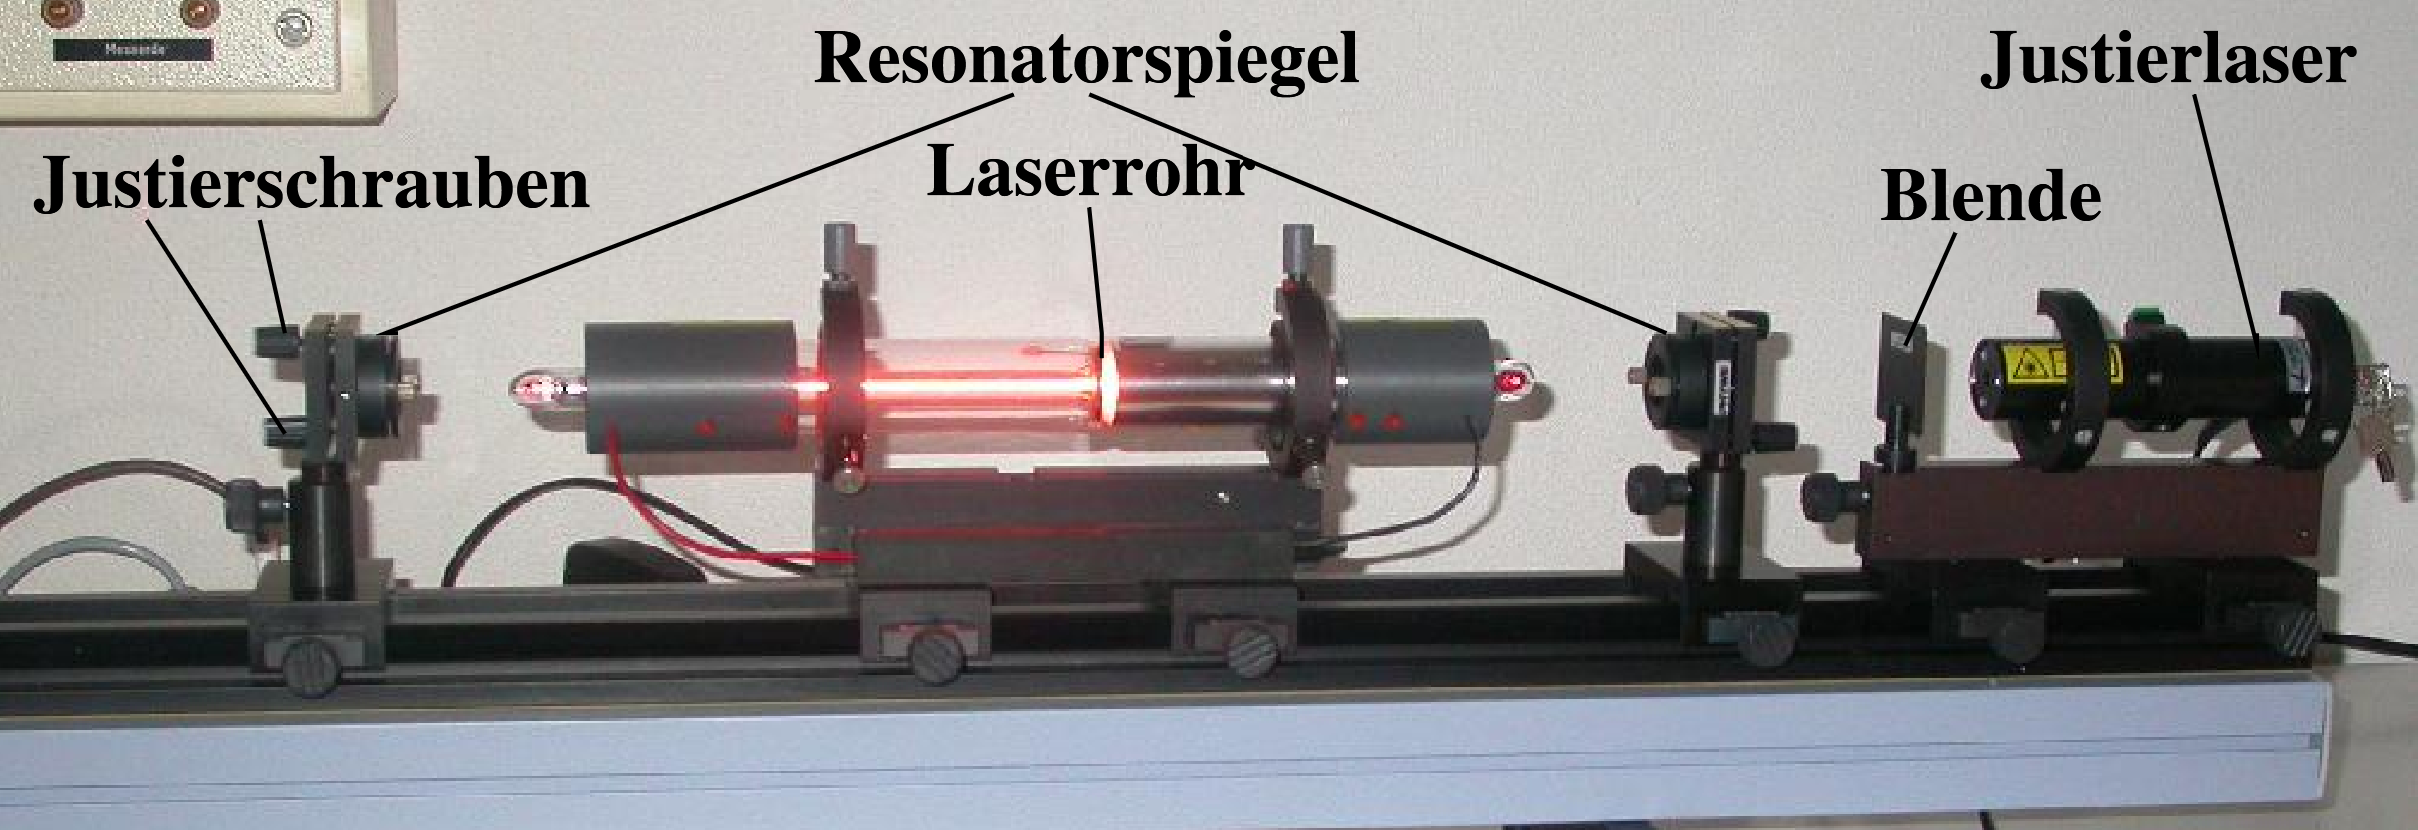
\includegraphics[width=\textwidth]{content/Aufbau_HeNe.png}
  \caption{Abbildung des genutzten grundlegenden Aufbaus wie im Versuch genutzt \cite{Anleitung_HeNe}.}
  \label{fig:Aufbau}
\end{figure}
Für die Justage stehen zwei Justierblenden zur Verfügung. Für die Messung der TEM-Moden ist ein eingespannter Wolframdraht mit einem Durchmesser von $d = 0,005$ genutzt. Für die Bestimmung der Polarisation wird ein, auf ein Grad einstellbarer,
Polarisator genutzt. Für die Bestimmung der Wellenlänge des Lasers werden zwei Gitter genutzt, eines mit einer Gitterkonstante von $12,5 \unit{\micro\meter}$ und eines mit einer Gitterkonstante von $10 \unit{\micro\meter}$.


\section{Durchführung}
\label{sec:Durchführung}
Zu Beginn der Durchführung des Versuchs muss der Aufbau justiert werden. Dazu wird das Laserrohr und die Resonatorspiegel auf der optischen Schiene platziert und mithilfe des Justierlasers ausgerichtet, so dass alle Reflexe die Mitte der
Justierblenden im Fadenkreuz treffen. Sobald das erreicht ist, wird der Justierlaser abgeschaltet. An dem Laserrohr ist eine Hochspannungsquelle angeschlossen, diese wird auf $6,5 \unit{\milli\ampere}$ eingestellt und eingeschaltet. Die Spiegel
und das Laserrohr werden anschließend einzeln Nachjustiert um eine möglichst hohe Leistung des HeNe-Lasers zu erreichen.

\subsection{Messung der Wellenlänge}
Zur Messung der Wellenlänge wird ein Gitter in den aus dem Resonator austretenden Strahl eingesetzt. Die Positionen der Interferenzmaxima, in dem entstehenden Interferenzmuster, werden mithilfe eine senkrecht zum Strahl verschiebbaren Photodiode
vermessen. Hierbei wird ebenfalls der Abstand der Photodiode zum Gitter aufgenommen. Dieser Schritt wird für zwei Gitter durchgeführt.

\subsection{Bestimmung der Polarisation}
Die Bestimmung der Polarisation erfolgt durch das einsetzen eines Polarisator im ausgekoppeltem Strahl. Unter Zuhilfenahme einer Photodiode wird die Intensität des durch den Polarisator tretenden Strahl gemessen. Diese Messung wird für
verschiedene Einstellungen des Polarisators in $4 \unit{\degree}$ Schritten durchgeführt.

\subsection{Vermessung der TEM-Moden}
Um die TEM-Moden zu isolieren wird der eingespannte Wolframdraht in den Strahl gebracht und bewegt bis eine Mode dominant sichtbar ist. Die Intensität dieser wird mit einer Photodiode entlang einer Achse in $1 \unit{\milli\meter}$ Schritten
gemessen. Dieser Vorgang wird für alle erreichbaren Moden wiederholt, in diesem Fall die $TEM_{00}$ und die $TEM_{10}$ Mode.

\subsection{Stabilität bei verschiedenen Resonatorlängen}
Um die Stabilität des Resonators zu prüfen wird der Abstand zwischen den Resonatorspiegeln vergrößert und alle Bestandteile des Lasers so nachjustiert, dass die Leistung maximal ist. Dieser Prozess wird so lange wiederholt bis das Ende der 
optischen Schiene erreicht ist oder der Laserprozess nicht mehr beginnt. Hierfür werden zwei Spiegelkombinationen genutzt. Ein planarer Spiegel und ein konvexer Spiegel mit einem Radius von $R = 1400 \unit{\milli\meter}$ sowie zwei konvexe 
Spiegel, ebenfalls mit einem Radius von $R = 1400 \unit{\milli\meter}$.